\documentclass{article}
\usepackage{amsmath}
\usepackage{graphicx}
\usepackage{float}

\begin{document}

\title{COMS 574 Final Project Report}
\author{Justin Stanley}

\maketitle

\section{Introduction}

For this project I conducted experiments analyzing the behavior of different classification models, including SVMs, decision trees, random forests, and neural networks.

\section{Experiments (Part 1)}

\subsection{Results}

\subsubsection{Cross-validation by method}

I used K-fold (K=5) and LOOCV cross validation to compare each classification method on each dataset. 100 trees are used for the random forest. The random forest has the strongest test accuracy on dataset 1, however took the longest time to train. This was especially long when LOOCV cross-validation is used, as the training time is quadratic in the number of samples. All classifiers performed significantly worse than dataset 1, suggesting dataset 2 contains more evenly distributed/mixed features. The random forest exhibited the strongest performance across each dataset.

The results are formatted by the following variables:
\begin{center}
    \begin{tabular}{l l}
        \textbf{Classifier} & $C$ \\
        \textbf{Validation method} & $V$ \\
        \textbf{Train accuracy} & $A_T$ \\
        \textbf{Train precision} & $P_T$ \\
        \textbf{Train recall} & $R_T$ \\
        \textbf{Train F1} & $F_T$ \\
        \textbf{Test accuracy} & $A_S$ \\
        \textbf{Test precision} & $P_S$ \\
        \textbf{Test recall} & $R_S$ \\
        \textbf{Test F1} & $F_S$ \\
    \end{tabular}
\end{center}

\begin{center}\textbf{Dataset 1}\end{center}
\begin{center}
\begin{tabular}{| l | c |  c | c | c | c | c | c | c | c |}
    \hline
    \textbf{C} & \textbf{V} & \textbf{$A_T$} & \textbf{$A_S$}
    & \textbf{$P_T$} & \textbf{$P_S$} & \textbf{$R_T$}
    & \textbf{$R_S$} & \textbf{$F_T$} & \textbf{$F_S$} \\
    \hline
    SVM & K-fold & 0.92 & 0.916 & 0.968 & 0.972 & 0.816 & 0.797 & 0.442 & 0.434 \\
    SVM & LOOCV  & 0.922 & 0.912 & 0.966 & 0.955 & 0.819 & 0.802 & 0.443 & 0.5 \\
    DecisionTree & K-fold & 1 & 0.917 & 1 & 0.876 & 1 & 0.904 & 0.5 & 0.444 \\
    DecisionTree & LOOCV & 1 & 0.921 & 1 & 0.885 & 1 & 0.906 & 0.5 & 0.5 \\
    RandomForest & K-fold & 1 & 0.963 & 1 & 0.965 & 1 & 0.933 & 0.5 & 0.474 \\
    RandomForest & LOOCV & 1 & 0.963 & 1 & 0.957 & 1 & 0.943 & 0.5 & 0.5 \\
    \hline
\end{tabular}
\end{center}

\begin{center}\textbf{Dataset 2}\end{center}
\begin{center}
\begin{tabular}{| l | c |  c | c | c | c | c | c | c | c |}
    \hline
    \textbf{C} & \textbf{V} & \textbf{$A_T$} & \textbf{$A_S$}
    & \textbf{$P_T$} & \textbf{$P_S$} & \textbf{$R_T$}
    & \textbf{$R_S$} & \textbf{$F_T$} & \textbf{$F_S$} \\
    \hline
    SVM & K-fold & 0.675 & 0.660 & 0.73 & 0.708 & 0.094 & 0.076 & 0.098 & 0.099 \\
    SVM & LOOCV  & 0.668 & 0.662 & 0.721 & 0.643 & 0.065 & 0.056 & 0.06 & 0.5 \\
    DecisionTree & K-fold & 1 & 0.593 & 1 & 0.427 & 1 & 0.459 & 0.5 & 0.219 \\
    DecisionTree & LOOCV & 1 & 0.584 & 1 & 0.405 & 1 & 0.425 & 0.5 & 0.5 \\
    RandomForest & K-fold & 1 & 0.662 & 1 & 0.531 & 1 & 0.395 & 0.5 & 0.222 \\
    RandomForest & LOOCV & 1 & 0.697 & 1 & 0.583 & 1 & 0.438 & 0.5 & 0.5 \\
    \hline
\end{tabular}
\end{center}

For simplification, the Precision, Recall, and F1 data are omitted from the remainder of the experiments, as they are not significantly related to the analysis of overfitting and underfitting.

\subsubsection{SVM Regularization}

For regularization experiments I manipulated the parameter $C$ used by the scikit-learn SVC. I tested the values $C=0.1, 1, 10, 50, 100, 1000$. I found that as the regularization constant increased, the SVC had better training and testing accuracy, however the model took slightly longer to train.

\begin{center}\textbf{Dataset 1}\end{center}
\begin{center}
\begin{tabular}{| l | c | c |}
    \hline
    \textbf{C} & \textbf{Accuracy (train)} & \textbf{Accuracy (test)} \\
    \hline
        0.1 & 0.893 & 0.889 \\
        1 & .920 & .919 \\
        10 & .923 & .925 \\
        50 & .933 & .933 \\
        100 & .941 & .931 \\
        1000 & .956 & .958 \\
    \hline
\end{tabular}
\end{center}

\begin{center}\textbf{Dataset 2}\end{center}
\begin{center}
\begin{tabular}{| l | c | c |}
    \hline
    \textbf{C} & \textbf{Accuracy (train)} & \textbf{Accuracy (test)} \\
    \hline
        0.1 & 0.654 & 0.654 \\
        1 & 0.673 & 0.664 \\
        10 & 0.733 & .699 \\
        50 & 0.756 & 0.695 \\
        100 & .766 & .719 \\
        1000 & .810 & 0.697 \\
    \hline
\end{tabular}\end{center}

\subsection{Decision tree splitting}

I analyzed the performance of GINI, entropy and log-loss methods for training decision trees and random forests. The random forest using entropy-based splitting performed best on dataset 1, while the random forest using either GINI or log-loss performed best on dataset 2.

\begin{center}\textbf{Dataset 1}\end{center}
\begin{center}
\begin{tabular}{| l | c | c | c |}
    \hline
    \textbf{Method} & \textbf{Split} & \textbf{Accuracy (train)} & \textbf{Accuracy (test)} \\
    \hline
        DecisionTree & GINI & 1 & .940 \\
        DecisionTree & Log-loss & 1 & .897 \\
        DecisionTree & Entropy & 1 & .939 \\
        RandomForest & GINI & 1 & .956 \\
        RandomForest & Log-loss & 1 & .96\\
        RandomForest & Entropy & 1 & .963 \\
    \hline
\end{tabular}
\end{center}

\begin{center}\textbf{Dataset 2}\end{center}
\begin{center}
\begin{tabular}{| l | c | c | c |}
    \hline
    \textbf{Method} & \textbf{Split} & \textbf{Accuracy (train)} & \textbf{Accuracy (test)} \\
    \hline
        DecisionTree & GINI & 1 & .602 \\
        DecisionTree & Log-loss & 1 & .597 \\
        DecisionTree & Entropy & 1 & .621 \\
        RandomForest & GINI & 1 & .686 \\
        RandomForest & Log-loss & 1 & .686 \\
        RandomForest & Entropy & 1 & .673 \\
    \hline
\end{tabular}
\end{center}

\subsection{Random forest tree count}

For this experiment I evaluated the performance of random forests with 10, 100, 500, 1000, and 10000 trees. The testing accuracy generally increased as the number of trees increased, as expected. The training time was significantly longer for the forests with 10000 trees.

\begin{center}\textbf{Dataset 1}\end{center}
\begin{center}
\begin{tabular}{| l | c | c |}
    \hline
    \textbf{Tree count} & \textbf{Accuracy (train)} & \textbf{Accuracy (test)} \\
    \hline
        10 & 0.999 & 0.958 \\
        100 & 1 & 0.961\\
        500 & 1 & 0.958\\
        1000 & 1 & 0.956 \\
        10000 & 1 & 0.965 \\
    \hline
\end{tabular}
\end{center}

\begin{center}\textbf{Dataset 2}\end{center}
\begin{center}
\begin{tabular}{| l | c | c |}
    \hline
    \textbf{Tree count} & \textbf{Accuracy (train)} & \textbf{Accuracy (test)} \\
    \hline
        10 & 0.979 & 0.651 \\
        100 & 1 & 0.677\\
        500 & 1 & 0.677\\
        1000 & 1 & 0.68 \\
        10000 & 1 & 0.68 \\
    \hline
\end{tabular}
\end{center}

\subsection{Summary}

By the experiments performed above, the strongest classifier for dataset 1 is a random forest training on entropy loss (test acc $0.963$), with 10000 trees (test acc $0.965$).

The strongest classifier for dataset 2 is an SVM with regularization constant $C=100$ with a test accuracy of $0.719$.

\section{Experiments (Part 2)}

\subsection{Hidden units}
For this experiment I evaluated the performance of the model with 12, 32, 64, and 128 units. The results are visualized in figure \ref{fig:units}. The results show the model accuracy converges fastest when 12 hidden units are used.

\begin{figure}[H]
    \centering
    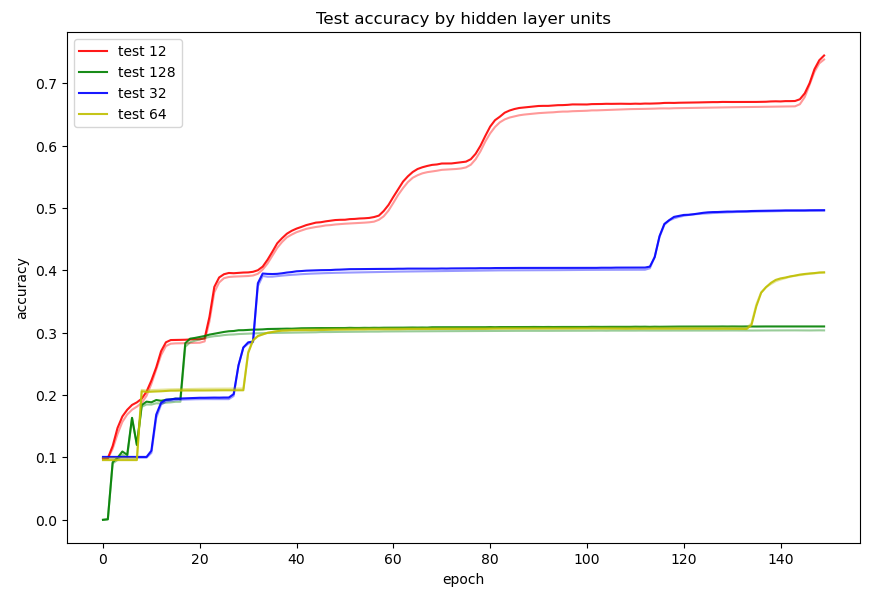
\includegraphics[width=0.8\textwidth]{part2/experiments/units/units.png}
    \label{fig:units}
    \caption{Network accuracy over time by hidden units}
\end{figure}

\subsection{Learning rate}
For this experiment I evaluated the performance of the model with learning rates of 0.001, 0.005, and 0.01. The results are visualized in figure \ref{fig:lr}. The results show the model accuracy converges fastest with a learning rate of 0.005, but finishes with the best accuracy at learning rate 0.005.

\begin{figure}[H]
    \centering
    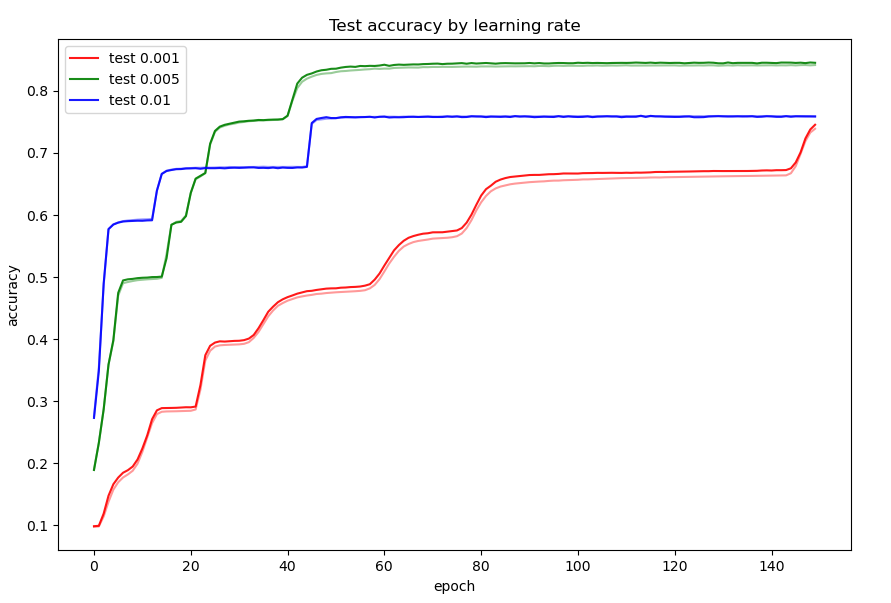
\includegraphics[width=0.8\textwidth]{part2/experiments/lr/lr_000.png}
    \label{fig:lr}
    \caption{Network accuracy over time by learning rate}
\end{figure}

\subsection{Regularization}
For this experiment I evaluated the performance of the model with different weight regularization. I tested L2 regularization multipliers of 0, 0.001, and 0.003. The results are visualized in figure \ref{fig:reg}. The results show the model accuracy converges fastest with no regularization, and performs generally worse as regularization increases.

\begin{figure}[H]
    \centering
    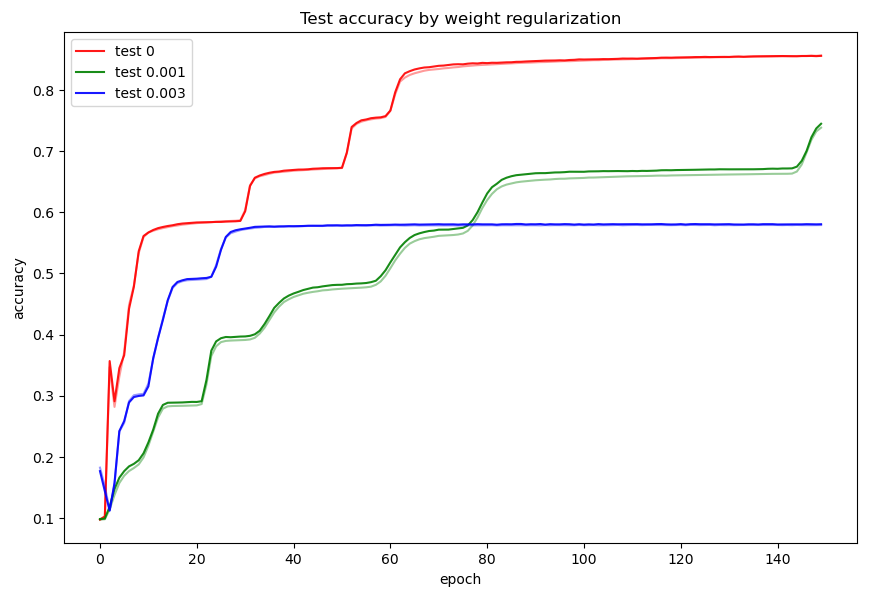
\includegraphics[width=0.8\textwidth]{part2/experiments/regularization/regularization.png}
    \label{fig:reg}
    \caption{Network accuracy over time by L2 regularization weight}
\end{figure}

\subsection{Activation}
For this experiment I evaluated the performance of the model with different activation functions. I tested the model using relu, sigmoid, and tanh activation. The results are visualized in figure \ref{fig:act}. The results show the model accuracy converges fastest with tanh activation, and slowest with sigmoid.

\begin{figure}[H]
    \centering
    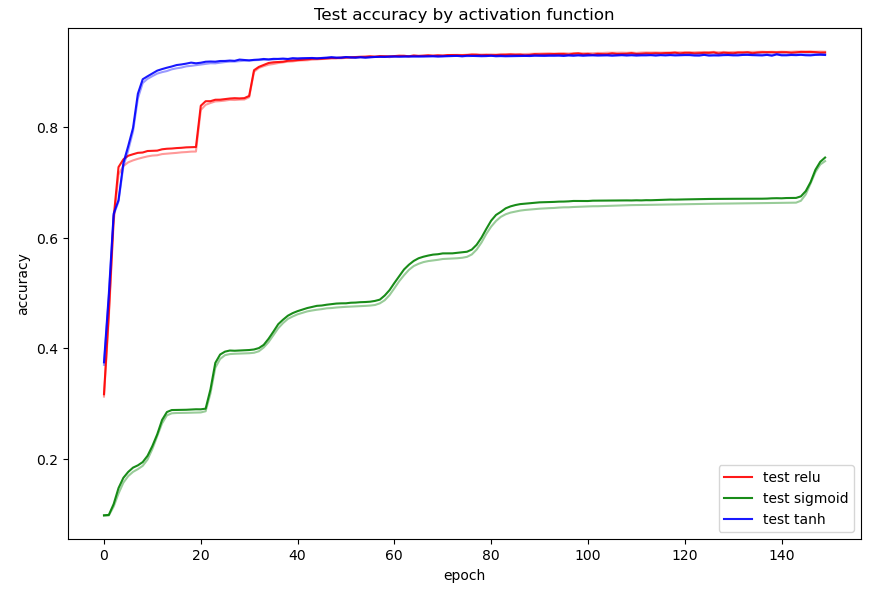
\includegraphics[width=0.8\textwidth]{part2/experiments/activation/activation.png}
    \label{fig:act}
    \caption{Network accuracy over time by activation function}
\end{figure}

\subsection{Summary}

By the experiments performed above, the final best model is one with 12 hidden units by 2 layers, tanh activation function, with learning rate 0.005 and no regularization.

\section{Supplementary materials}

\end{document}
